\subsection{Events}

\begin{table}[h]
	\centering
	\resizebox{\columnwidth}{!}{
	\begin{tabular}{||c | c | c | c||} 
		\hline
		\textbf{Event} & \textbf{System Response} & \textbf{Source} & \textbf{Type}\\
		\hline\hline
Luminosity detector OFF & Power the lamp & Environment & Asynchronous\\\hline
LED failure detector ON & Notify remote system & Local system & Asynchronous\\\hline
Motion detected & Turn on the lamp & User & Asynchronous\\\hline
Requested to turn on the lamp & Turn on the lamp & Base station & Asynchronous\\\hline
Update system information & Send data to remote system & Base station & Asynchronous\\
		\hline
	\end{tabular}
	}		
	
	\caption{Local system events.}
	\label{table:ls_events}
\end{table}

\subsection{Use Cases}

\begin{figure}[ht]
	\centering
	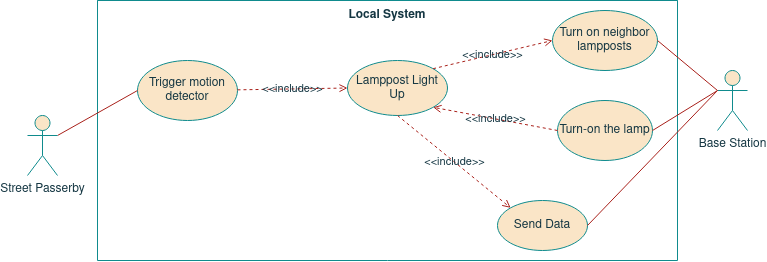
\includegraphics[width=1\textwidth]{/04local_system/LS_UseCase}
	\caption{Local system use cases.}
	\label{fig:ls_use_cases}
\end{figure}

\subsection{State Chart}

\begin{figure}[ht]
	\centering
	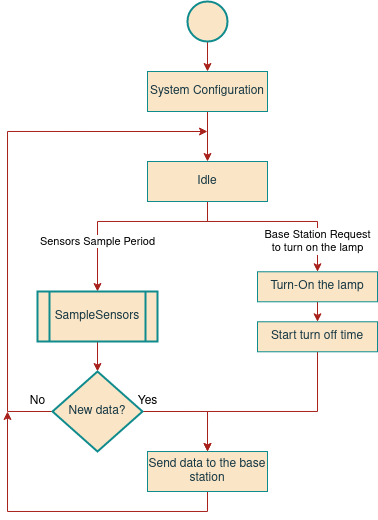
\includegraphics[width=.65\textwidth]{/04local_system/LS_StateChart}
	\caption{Local system state chart.}
	\label{fig:ls_state_chart}
\end{figure}

\subsection{Sequence Diagram}

\begin{figure}[ht]
	\centering
	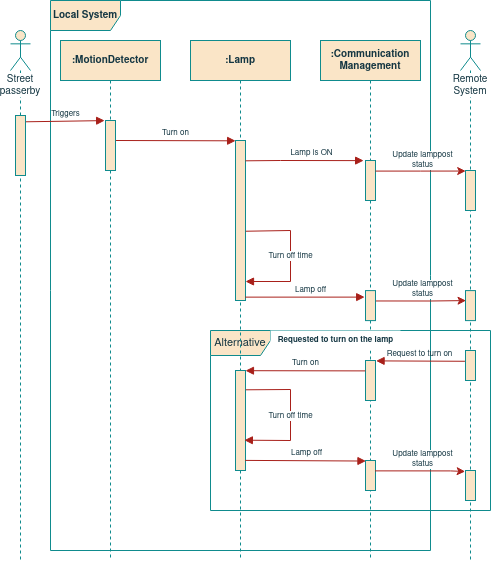
\includegraphics[width=.85\textwidth]{/04local_system/LS_SeqDiagram}
	\caption{Local system sequence diagram.}
	\label{fig:ls_seq_diagram}
\end{figure}